\chapter{New Material For Supervised Learning}
\chapterauthor{Jeff Yoshimi}

\section{Finding A Linear Decision Boundary Manually}

Suppose we have a simple pattern association task which classifies six input vectors into two categories, using bipolar outputs (1 means the input is in the category, -1 means it is not in the category). The task is defined by the table shown in  figure \ref{simpleTask}.  We can also plot the input space, labeling points by their target values. Notice that this task is linearly separable. 

\begin{figure}[h]
\centering
\includegraphics[scale=.6]{./images/decisionBoundary.png}
\caption{A classification task that can be solved by hand.}
\label{simpleTask}
\end{figure}

How do we design a neural network to solve this problem? First we build an appropriate network. It will have two input nodes and one output node. We make the output node a binary unit with upper bound 1, lower bound -1, and threshold 0. So the output node will output a 1 if weighted input is greater than 0, and -1 otherwise.

We now focus on the three adjustable parameters of the network: the two weight strengths $w_{1,3}$ and $w_{2,3}$, and the bias $b_3$ of the output node. A learning algorithm can learn this decision boundary automatically, but we can also just use algebra to find the right boundary.

To do this, we need to know how to make a network produce a particular decision boundary. The decision boundary in this case is the set of points in the $x_1 - x_2$ plane such that weighted input $n_3 = 0$. Points on one side of this line will produce  $n_3 > 0$, and so the output will be 1. Points on the other side of the line will produce an output of -1. (A geometric way of understanding what the decision boundary is included below). So we want to set the weights and bias so that this decision boundary has slope $-1$ and an $x_2$-intercept of $1$. The equation for the weighted input to neuron 3 is:
\begin{eqnarray*}
n_3 =  w_{1,3} x_1 + w_{2,3}  x_2 + b_3
\end{eqnarray*}
Since the set of points where $n_3$ is 0 is the decision boundary, we set $n_3$ to 0:
\begin{eqnarray*}
0 = x_1 w_{1,3} + x_2 w_{2,3} + b_3
\end{eqnarray*}
Now we solve for $x_2$:
\begin{eqnarray*}
x_2 = -\frac{w_{1,3}}{w_{2,3}} x_1  - \frac{b_3}{w_{2,3}}
\end{eqnarray*}
Notice that this is an equation for a line in the plane, that is, an equation of the form $y = mx + b$, where $m = -w_{1,3} / w_{2,3}$, and $b =  -b_3 / w_{2,3}$. To make this clear, here is the same equation, with boxes around the slope and intercept terms:
\begin{eqnarray*}
x_2 =  \boxed{-\frac{w_{1,3}}{ w_{2,3}}} x_1 - \boxed{\frac{b_3}{w_{2,3}}}
\end{eqnarray*}

Just by visual inspection of figure \ref{simpleTask}, we can see that the slope of a good decision line would be about -1, and a $x_2$-intercept of about 1. This is enough to build a network to solve the problem. The boxed values above correspond to the slope and $x_2$-intercept of the equation for the decision boundary. Our goal is to produce a network with a decision boundary like the one shown in figure \ref{simpleTask}, with slope -1 and $x_2$-intercept of 1. That is ,we want:
\begin{eqnarray*}
-\frac{w_{1,3}}{w_{2,3}} = -1 \\
-\frac{b_3 }{w_{2,3}} = 1 \\
\end{eqnarray*}
We can set the weight and bias values to do this in various ways. For example, we can set both weights to 1, so that the slope is -1. Then to set $x_2$-intercept to 1, we set $b_3$ to -1. So then our network parameters are:
\begin{eqnarray*}
w_{1,3}  = 1 \\
w_{2,3}  = 1 \\
b_3  = -1 \\
\end{eqnarray*}

This should give us the right results. Try building a network with these properties and see if it succeeds in the classification task  shown in figure \ref{simpleTask}.

So to summarize: the decision boundary, which separates the input space into different classes, shifts in two key ways: (1) its slope, determined by the ratio of the weights $-\frac{w_{1,3}}{w_{2,3}}$, and (2) its intercept, which is shifted left or right by the bias $b_3$, scaled by the weight $w_{2,3}$, as seen in the term $-\frac{b_3}{w_{23}}$.

\section{Geometric intuition about the decision boundary}

% Another useful feature of this discussion is it helps us think about what the weight vector and bias do geometrically

In the neural network discussed above, with two inputs and one output, the weighted input $n_3$ to the output node is given by the equation:
\begin{eqnarray*}
n_3 = w_{1,3} x_1 + w_{2,3} x_2 + b_3
\end{eqnarray*}
The threshold for classification, that is the decision boundary, can be visualized as a horizontal plane, typically at $n_3 = 0$ (as in our example), which intersects the surface defined by the equation above. This intersection is normal (that is, perpendicular) to the vector $(w_{1,3}, w_{2,3})$. To see this, note that (assuming a bias of 0), for any input $(p_1,p_2)$ for which $n_3 = 0$, $(w_{1,3}, w_{2,3}) \bullet  (p_1,p_2) = 0$, so the weight vector is orthogonal to any point on the decision boundary.

The bias $b_3$ shifts this plane vertically along the $n_3$-axis without affecting its orientation, while the weights determine the plane’s tilt. As you can see visually in the figure, inputs below the decision boundary will produce a negative net-input which is below threshold, while those above the decision boundary will produce a positive net-input which is above threshold.

This discussion provides a link between the discussion of regression surfaces and decision boundaries. The weighted input corresponds to a regression surface for a linear output node. When we apply a threshold, this surface intersects another surface representing the threshold (the function $z = \theta$, with $\theta = 0$ in this case). The line of intersection between these two surfaces is the decision boundary

\begin{figure}[h]
\centering
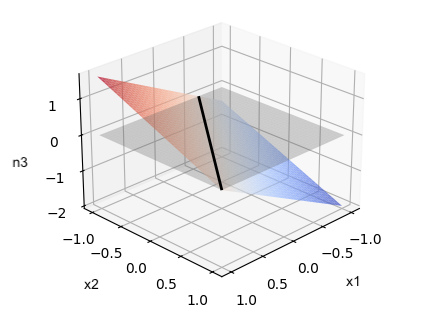
\includegraphics[scale=1.0]{./images/decisionLinePlanes.png}
\caption{A decision boundary as the intersection of two surfaces. Red colors correspond to net inputs that are above 0; blue colors correspond to net inputs that are below 0.}
\label{decisionLineSurface}
\end{figure}

